\documentclass{article}

\usepackage{amsmath,amssymb}
\usepackage{fullpage}
\usepackage{enumerate}
\usepackage{hyperref}
\usepackage{graphicx}
\graphicspath{{../logos/}}


\begin{document}

\setlength{\tabcolsep}{6pt}
\begin{center} \begin{tabular}{cccc}
	% set heights below to 43pt if fullpage not used
	
\includegraphics[height=56pt]{SAMF_logo.jpg} &
	
\includegraphics[height=56pt]{SAICA_logo.jpg} &
	
\includegraphics[height=56pt]{OM_Logo_Stacked_Vignette_on_White_RGB.jpg} &
	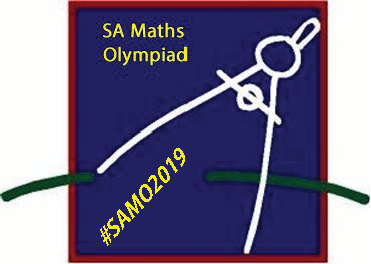
\includegraphics[height=56pt]{SAMO2019.png}
\end{tabular} \end{center}


\bigskip


\begin{center}
\textbf{\Large Senior Monthly Problem Set}
\\ \vspace{1em}
\textbf{\large Due: 28 February 2020}
\end{center}

\begin{enumerate}

\medskip
\item % Problem source
Let $ABC$ be a triangle with orthocentre $H$, such that $AB<BC$ and $\angle BAC < 90^\circ$. Let the circle $\Gamma$ centred at $B$ and passing through $A$ intersect $AC$ again at $D$. The circumcircle of $\triangle BCD$ intersects $\Gamma$ again at $E$. $ED$ and $BH$ intersect at $F$. Prove that $BD$ is tangent to the circumcircle of $\triangle DHF$.


\medskip
\item % IMO Long List 1992 Q75
Find all positive integers $n$ that can be written in the form:
$$n = \lfloor m + \sqrt{m} + \frac{1}{2} \rfloor$$
where $m$ is also a positive integer.

\medskip
\item


\medskip
\item
An $8 \times 8$ chessboard is divided into several regions by 13 straight lines. Can the lines be placed in such a way that each region contains at most 1 centre of the original 64 squares?


\medskip
\item


\medskip
\item % Mongolia 2008 TST Day 3 Q3
Show that there are only finitely many solutions $(x, y) \in \mathbb{N}^2$ to the equation
$$\sum_{i = 1}^{m} (x + i)^n = \sum_{i = 1}^{m} (y + i)^{2n}$$
where $m, n \in \mathbb{N} \setminus \{1\}$ are given constants.


\medskip
\item




\medskip
\item


\end{enumerate}


\vfill
\textbf{\Large Email submission guidelines}
\begin{itemize}
	\item Email your solutions to \href{mailto:samf.training.assignments@gmail.com}{\texttt{samf.training.assignments@gmail.com}}.
	\item In the subject of your email, include your name and the level of the assignment (Beginner, Intermediate or Senior).
	\item Submit each question in a single separate PDF file (with multiple pages if necessary), with your name and the question number written on each page.
	\item If you take photographs of your work, use a document scanner such as Office Lens to convert to PDF.
	\item If you have multiple PDF files for a question, combine them using software such as PDFsam.
\end{itemize}

\end{document}